%%%%%%%%%%%%%%%%%%%%%%%%%%%%%%%%%%%%%%%%%%%%%%%%%%%%%%%%%%%%%%%%%%%%%%%%%%%%%%%
% Chapter 'Absorption - Ethanol - ionic liquid [MMIM]+[(CH3)2PO4]-'
%%%%%%%%%%%%%%%%%%%%%%%%%%%%%%%%%%%%%%%%%%%%%%%%%%%%%%%%%%%%%%%%%%%%%%%%%%%%%%%
\subsection{Ionic liquid [MMIM]+[(CH3)2PO4]-}
%
%%%%%%%%%%%%%%%%%%%%%%%%%%%%%%%%%%%%%%%%%%%%%%%%%%%%%%%%%%%%%%%%%%%%%%%%%%%%%%%
%%%%%%%%%%%%%%%%%%%%%%%%%%%%%%%%%%%%%%%%%%%%%%%%%%%%%%%%%%%%%%%%%%%%%%%%%%%%%%%
\subsubsection{UniquacFixedDu - ID 1}
%
\begin{tabular}[l]{|lp{11.5cm}|}
\hline
\addlinespace

\textbf{Sorbent:} & ionic liquid \\
\textbf{Subtype:} & [MMIM]+[(CH3)2PO4]- \\
\textbf{Refrigerant:} & Ethanol \\
\textbf{Equation:} & UniquacFixedDu \\
\textbf{ID:} & 1 \\
\textbf{Reference:} & Kato, Ryo; Gmehling, Jürgen (2005): Measurement and correlation of vapor–liquid equilibria of binary systems containing the ionic liquids [EMIM][(CF3SO2)2N], [BMIM][(CF3SO2)2N], [MMIM][(CH3)2PO4] and oxygenated organic compounds respectively water. In: Fluid Phase Equilibria 231 (1), S. 38–43. DOI: 10.1016/j.fluid.2005.01.002. \\
\textbf{Comment:} & None \\

\addlinespace
\hline
\end{tabular}
\newline

\textbf{Equation and parameters:}
\newline
%
Pressure $p$ in $\si{\pascal}$ is calculated depending on molar fraction of refrigerant in the liquid phase $x_1$ in $\si{\mole\per\mole}$, temperature $T$ in $\si{\kelvin}$, and vapor pressure $p_\mathrm{sat,1}$ in $\si{\pascal}$ by:
%
\begin{equation*}
\begin{split}
p &=& \gamma_1 x_1 p_\mathrm{sat,1} & \quad\text{, and} \\
\gamma_1 &=& \exp \left( \ln \left( \nicefrac{\Phi_1}{x_1} \right) + q_1 \nicefrac{z}{2} \ln \left( \nicefrac{\Theta_1}{\Phi_1} \right) + l_1 - \nicefrac{\Phi_1}{x_2} \left( x_1 l_1 + x_2 l_2 \right) + \Gamma \right) & \quad\text{, and} \\
\Gamma &=& - q_1 \ln \left( \Theta_1 + \Theta_2 \tau_{21} \right) + q_1 - q_1 \left( \frac{\Theta_1}{\Theta_1 + \Theta_2 \tau_{21}} + \frac{\Theta_2 \tau_{12}}{\Theta_1 \tau_{12} + \Theta_2} \right) & \quad\text{, and} \\
\tau_{ij} &=& \exp \left( \nicefrac{\Delta u_{ij}}{R T} \right) & \quad\text{, and} \\
l_i &=& \nicefrac{z}{2} \left( r_i - q_i \right) \left(r_i - 1 \right) & \quad\text{, and} \\
\Theta_i &=& \frac{q_i x_i}{\sum_{j=1}^{2} q_j x_j} & \quad\text{, and} \\
\Phi_i &=& \frac{r_i x_i}{\sum_{j=1}^{2} r_j x_j} & \quad\text{, and} \\
x_2 &=& 1 - x_1  & \quad\text{.} \\
\end{split}
\end{equation*}
%
The parameters of the equation are:
%
\begin{longtable}[l]{lll|lll}
\toprule
\addlinespace
\textbf{Par.} & \textbf{Unit} & \textbf{Value} &	\textbf{Par.} & \textbf{Unit} & \textbf{Value} \\
\addlinespace
\midrule
\endhead

\bottomrule
\endfoot
\bottomrule
\endlastfoot
\addlinespace

$\Delta u_{12}$ & $\si{\joule\per\mole}$ & -5.866000000e+02 & $\Delta u_{21}$ & $\si{\joule\per\mole}$ & -2.027500000e+03 \\
$r_{1}$ & - & 2.105000000e+00 & $r_{2}$ & - & 7.162000000e+00 \\
$q_{1}$ & - & 1.972000000e+00 & $q_{2}$ & - & 5.844000000e+00 \\
$z$ & - & 1.000000000e+01 & & &  \\

\addlinespace\end{longtable}

\textbf{Validity:}
\newline
Equation is approximately valid for $353.15 \si{\kelvin} \leq T \leq 353.15 \si{\kelvin}$.
\newline

\textbf{Visualization:}
%
\begin{figure}[!htp]
{\noindent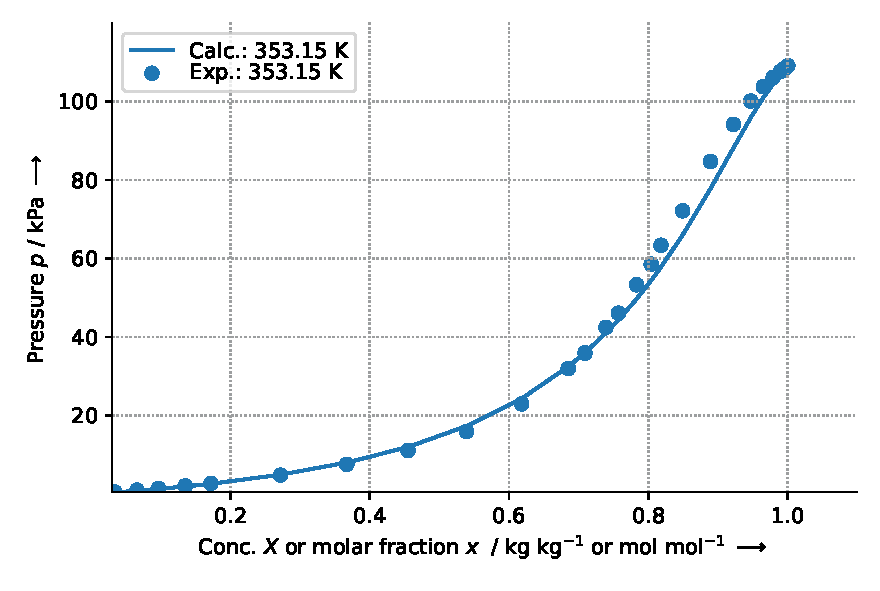
\includegraphics[height=10cm, keepaspectratio]{figs/abs/abs_Ethanol_ionic_liquid_[MMIM]+[(CH3)2PO4]-_UniquacFixedDu_1.pdf}}
\end{figure}
%

To generate the figure, the following refrigerant functions were selected:
\begin{itemize}
\item Vapor pressure: VaporPressure\_EoS1 - ID 1
\item Saturated liquid density: SaturatedLiquidDensity\_EoS1 - ID 1
\end{itemize}

The uncertainity of the experimental data is:
\begin{itemize}
\item Data source $\,\to\,$ Data was taken from table
\end{itemize}

The mean absolute percentage error (MAPE) between the experimental and calculated data results in 5.22\%.
\FloatBarrier
\newpage
%%%%%%%%%%%%%%%%%%%%%%%%%%%%%%%%%%%%%%%%%%%%%%%%%%%%%%%%%%%%%%%%%%%%%%%%%%%%%%%
